\documentclass{beamer}

\title{Renewing Motor Box Seals}
\author{Ryan Bayes}

\begin{document}
\frame{\maketitle}

\begin{frame}{Motivation}
\begin{columns}
\column{0.55\textwidth}
\begin{itemize}
\item Know that the UI radon seal is not great
\item Leak rate is significantly reduced through the used of nitrogen bags
	\begin{itemize}
	\item<alert@1> Isolation bag around full UI has produced low radon monitor rates (before pump)
	\item<alert@2> Isolation bags around problematic features reduced rate relative to none
	\end{itemize}
	\end{itemize}
\column{0.5\textwidth}
\includegraphics<1>[width=\textwidth,angle=180]{IMG_4523.jpg}
\includegraphics<2>[width=0.8\textwidth]{UIView.png}
\end{columns}
\begin{itemize}
\item Main sources are;
	\begin{itemize}
	\item North siderope motor box 
	\item East rope extension box
	\end{itemize}
\item Both require o-ring require o-ring replacement
	\begin{itemize}
	\item Reduce nitrogen use by the experiment
	\item Restore functionality of North Motor box (bag cuts off access)
	\end{itemize}
\end{itemize}
\end{frame}

\begin{frame}{Summary of Prior Leak Checking Campaigns}
	\begin{table}
	\begin{tabular}{r|c|c|c}
	Feature & Status & Leak (mbar L/s)& Date\\
	East and west motor box & good & $< 2\times10^{-8}$ & June 2023 \\
	West extension box seal & good & $< 10^{-10}$ & June 2023 \\
	South motor box outer seal & pass & $5\times10^{-7}$ & June 2023 \\
	South motor box inner seal & fail &  $1.4\times10^{-5}$ & July 2023 \\
	South exten. box outer seal & fail &  $< 10^{-5}$ & June 2023 \\
	South exten. box inner seal & pass &  $2\times10^{-9}$ & July 2023 \\
	North motor box & fail &  $ > 10^{-4}$ & Oct 2019 \\
	North exten. box & pass&  $ < 10^{-9}$ & June 2023 \\
	East extension box seal & fail & $ > 10^{-4}$ & Oct 2019 \\
	\end{tabular}
	\end{table}
	\begin{itemize}
	\item CF flanges checked with helium/Argon sniffer
		\begin{itemize}
		\item Neck tube base flanges (Leaks observed and corrected)
		\item Level sensor flanges (no leaks observed)
		\item CF flanges on motor box (motor, electrical feedthroughs; no leaks)
		\end{itemize}
	\item Gloves tested by pumping and purging with N$_{2}$
		\begin{itemize}
		\item East gloves shown to leak, South and West gloves good.
		\end{itemize}
	\end{itemize}
\end{frame}

\begin{frame}{Proposed Intervention}
\begin{columns}
\column{0.65\textwidth}
\begin{itemize}
\item Detector at low voltage
\item Connect N$_{2}$ source to UI to "flush" UI
\item Remove bag from North Motor Box/East Extension Box
\item Remove cover from box
\item Examine/replace O-rings 
\item Replace box cover
\end{itemize}
\column{0.35\textwidth}
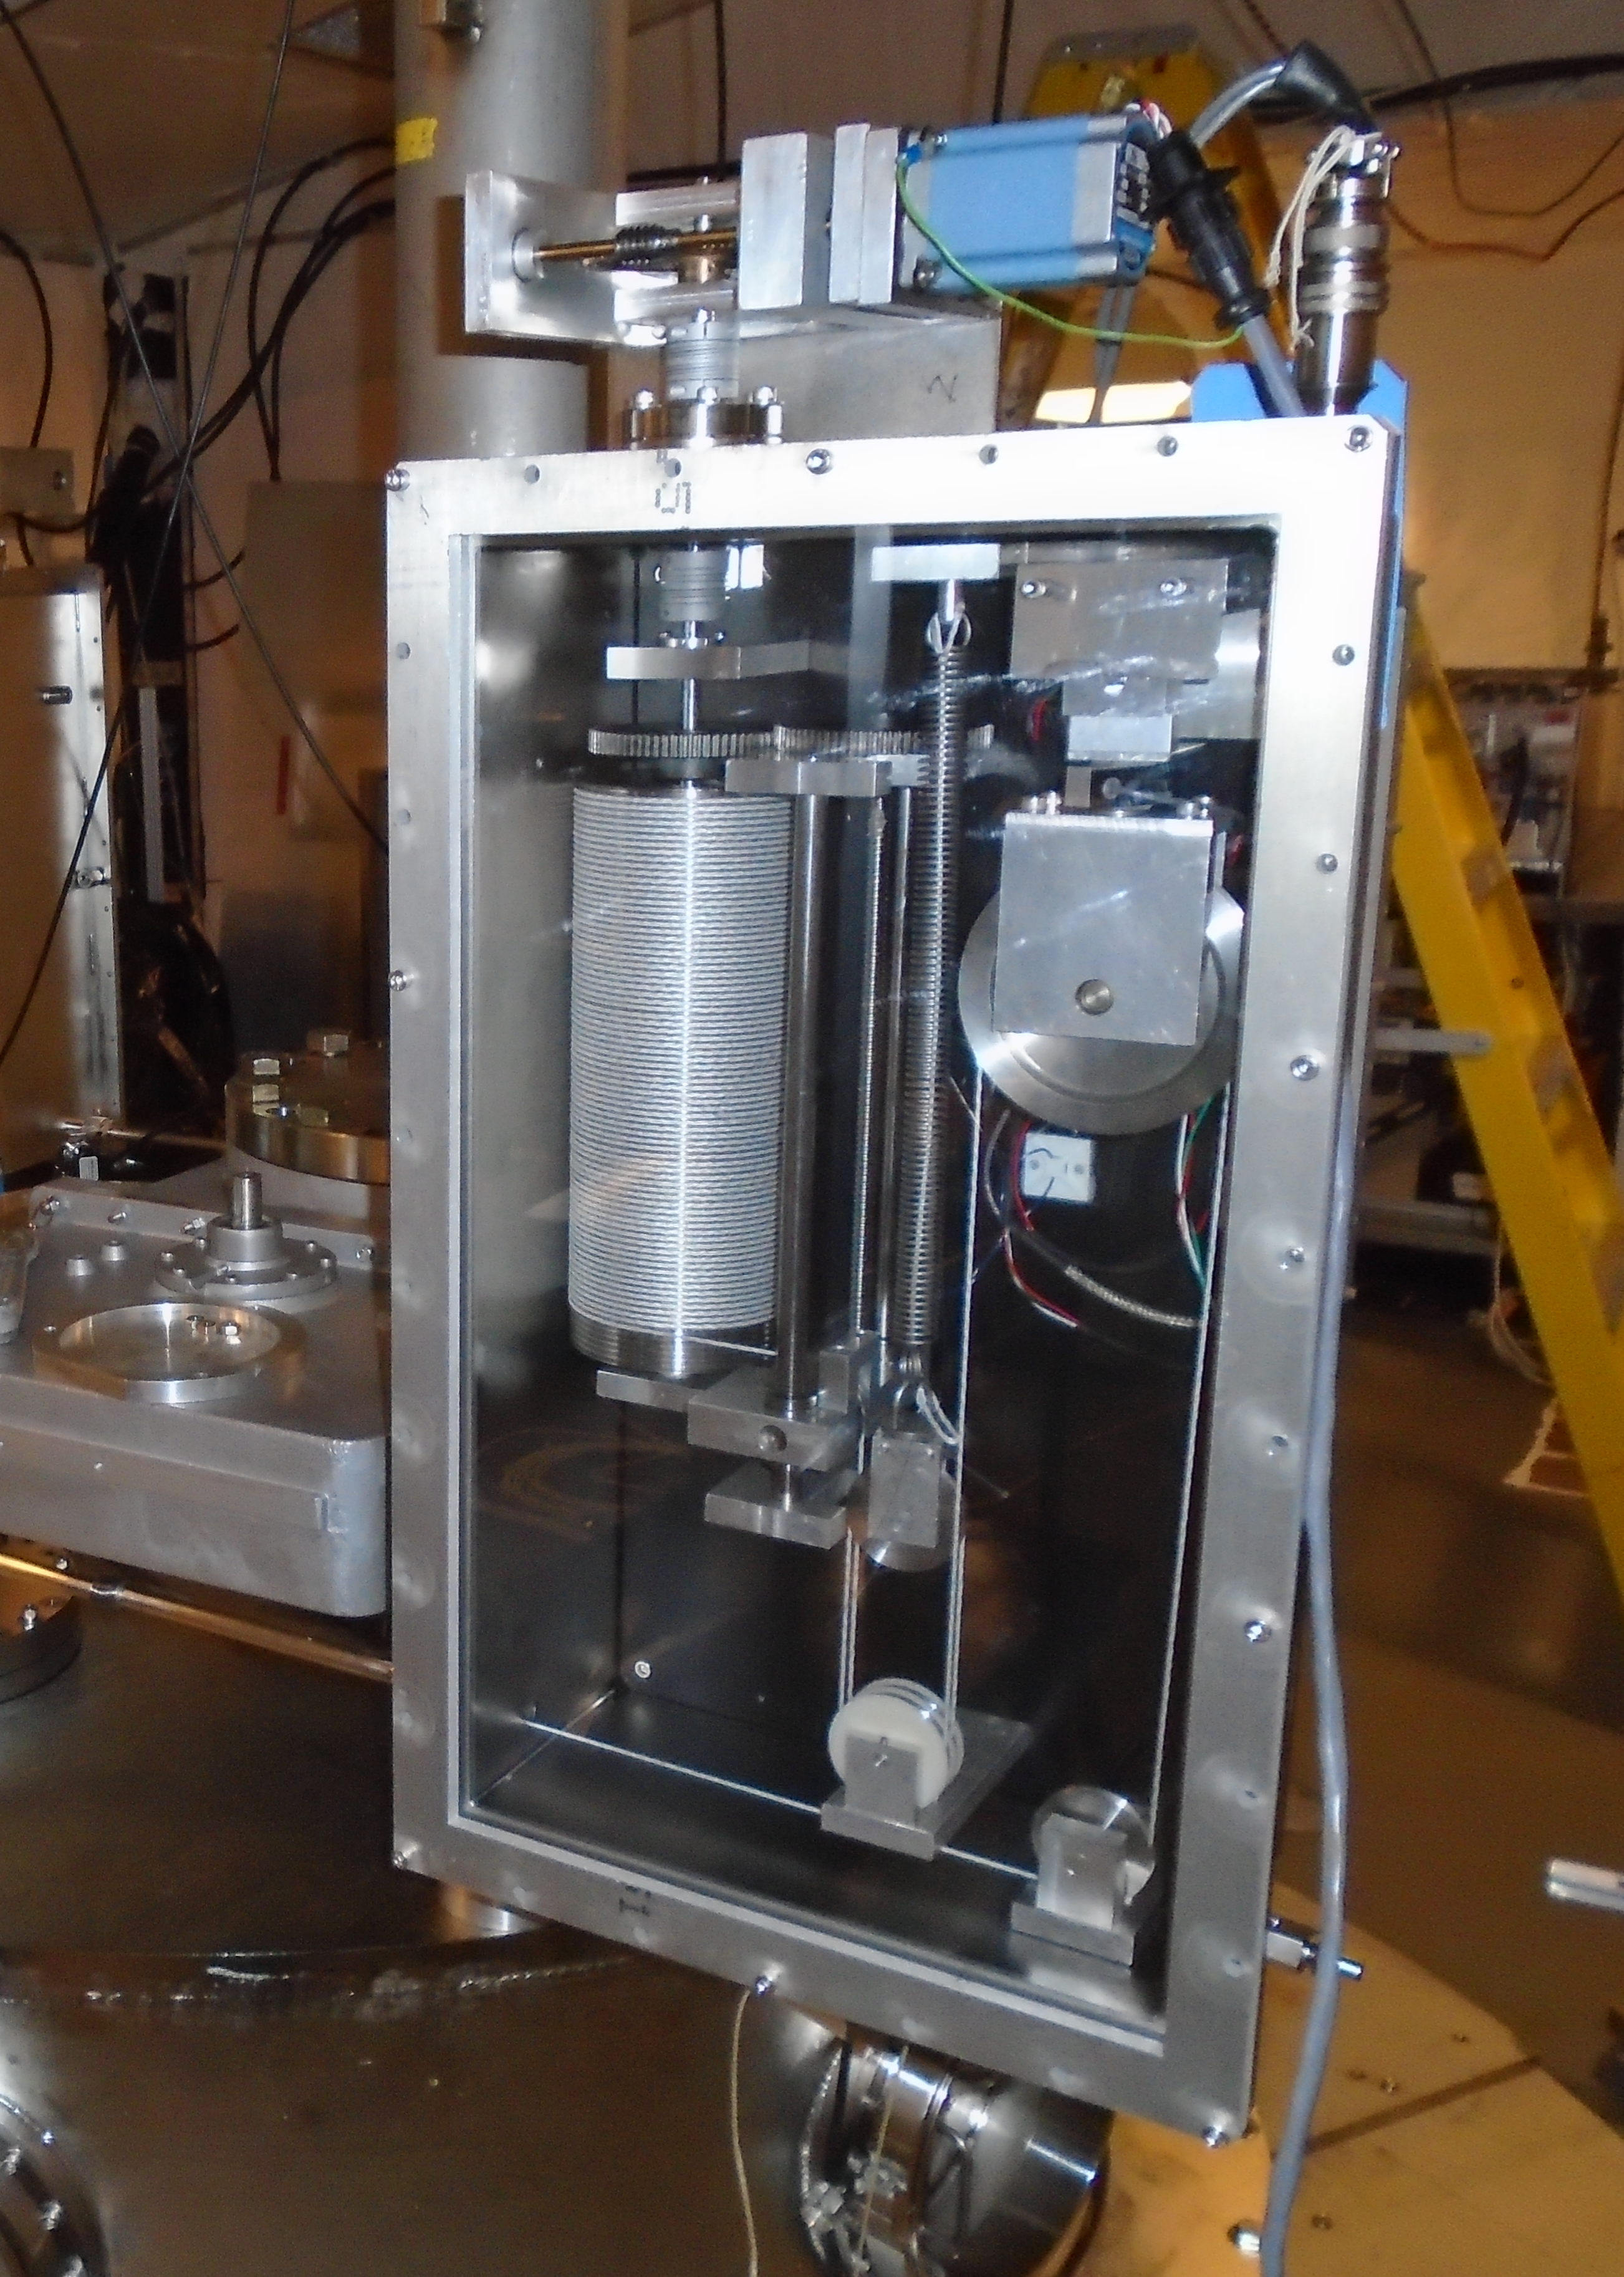
\includegraphics[width=\textwidth]{EastropeWindow.png}
\end{columns}
\vspace{-0.5cm}
\begin{block}{Radon mitigation}
\begin{itemize}
\item Keep the UI at positive pressure by adding nitrogen to UI (monitor through DeltaV)
\item Purge air from box after sealing by pulling air from motor box using auxiliary port
	\begin{itemize}
	\item Motor box is 35 L 
	\end{itemize}
\item Restrict air flow path size to less than the 1/2" port available
\end{itemize}
\end{block}

\end{frame}

\begin{frame}{Additional Steps}
	\begin{block}{Inner o-ring on South Motor Box}
		\begin{itemize}
		\item TEV o-ring bad; Viton o-ring "good" but emanates radon
		\item Replacing TEV o-ring could remove radon source
		\end{itemize}
	\end{block}
	\begin{block}{Outer o-ring on South Extension Box}
		\begin{itemize}
		\item TEV o-ring good; Viton bad 
		\item Unknown if this is damage or displacement
		\item TEV o-ring seal requires more torque; can relax with time
		\item Opening the box to inspect/rInn.
		eplace Viton o-ring will improve stability
		\end{itemize}
	\end{block}
\end{frame}

\begin{frame}{Neck Tube Radon Mitigation}
	\begin{columns}
	\column{0.7\textwidth}
	\begin{itemize}
	\item HV feedthroughs are "known" to be radon permiable
		\begin{itemize}
		\item Attempted isolation test but inconclusive
		\item Two isolation bags clearly hold pressure
		\item Two others are not so obvious (but that may be a flow problem)
		\end{itemize}
	\item Seal cannot be improved without completely changing the connection plate
	\item May need another attempt at isolation bags
	\item Increased pressure could improve isolation measure (get that by removing the large bags)
	\item Could improve the material; use aluminized mylar
	\end{itemize}
	\column{0.3\textwidth}
	\includegraphics[width=\textwidth]{NeckTubeFeedthrough.png}
	
	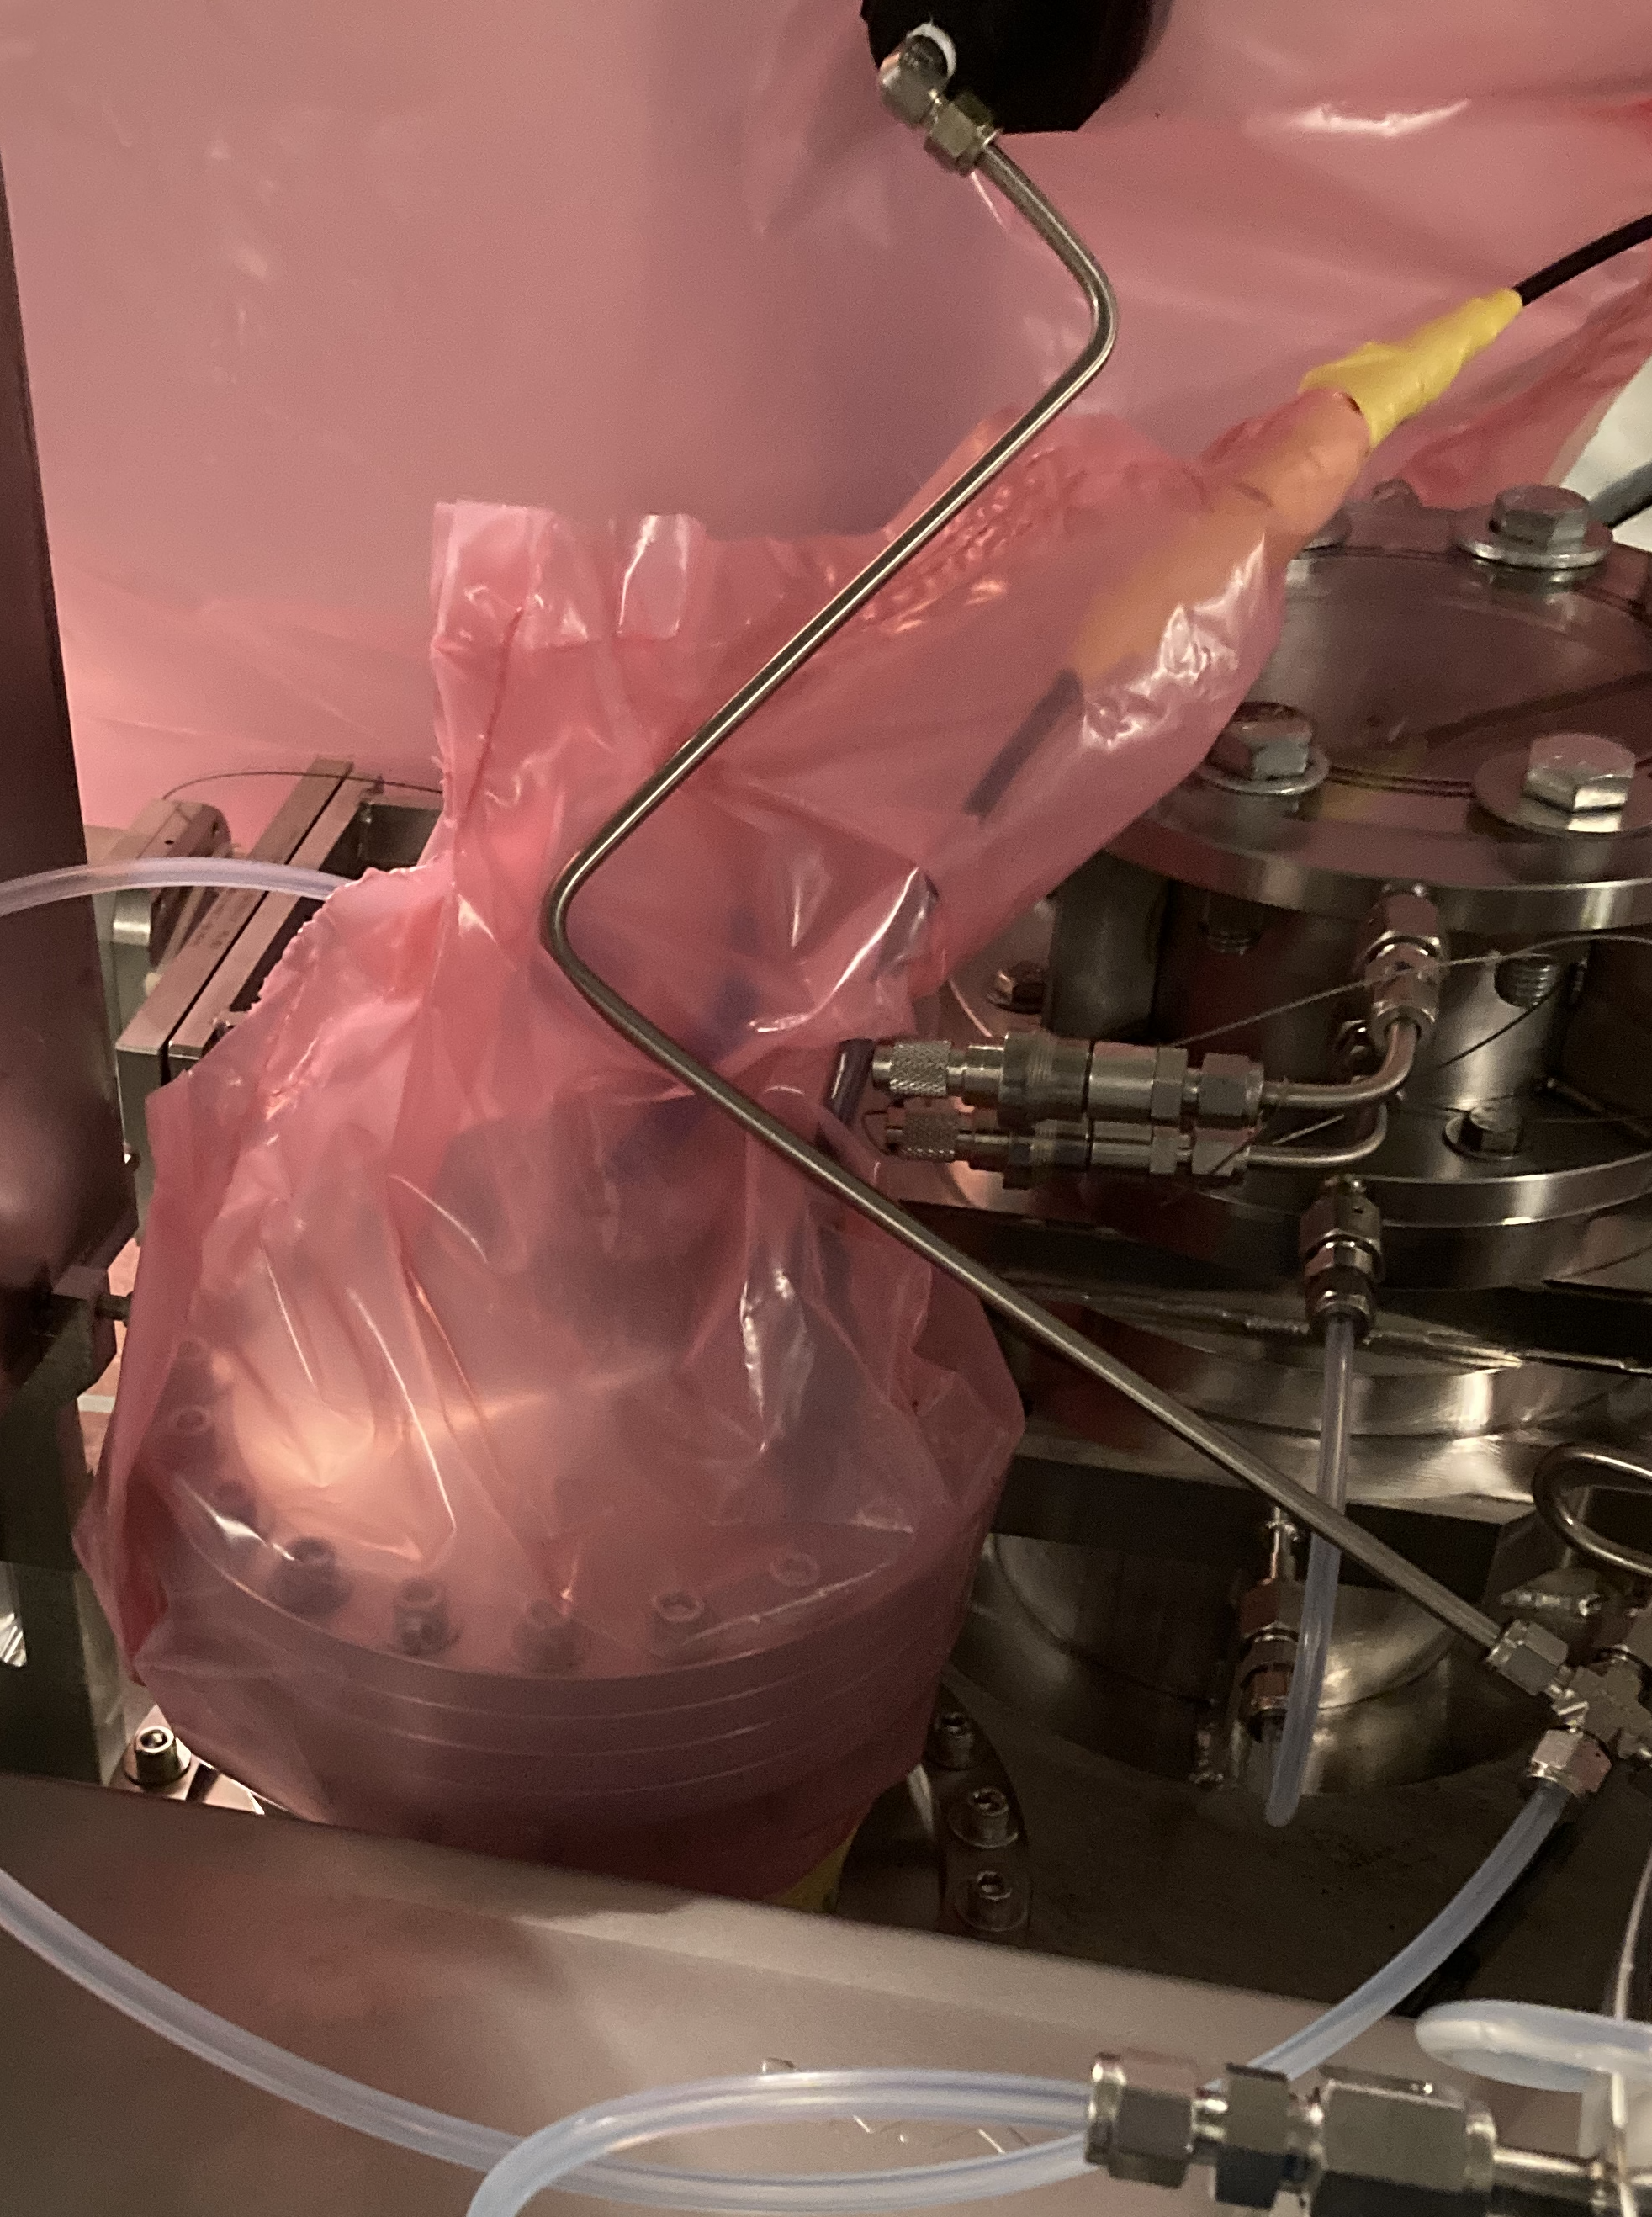
\includegraphics[width=\textwidth]{BaggedWestNeckTube.png}
	\end{columns}
	
\end{frame}

\begin{frame}{Summary}
	\begin{itemize}
	\item UI is known to leak radon
		\begin{itemize}
		\item $10^{-4}$ suppression relative to air from UI gas assays
		\item Radon monitor assays give a (much) higher number
		\end{itemize}
	\item Current solution is not sufficient
		\begin{itemize}
		\item Push to complete calibration program makes full UI bag problematic
		\item Current isolation bags interfere with side rope motor box operation
		\item Current bags are not as good as full bag (something is missing)
		\item N$_{2}$ use is restrictive; unclear if we can add further bags and maintain function
		\end{itemize}
	\item Propose to replace radon seals on selected motor box
		\begin{itemize}
		\item North Motor box and East Extension boxes need both o-ring sets replaced
		\item South motor box needs inner o-ring replaced
		\item South extension box needs outer o-ring replaced
		\end{itemize}
	\item Isolation bags on neck tubes should be more efficient without side rope isolation bags
		\begin{itemize}
		\item Some improvements could be considered there
		\end{itemize}
	\end{itemize}
\end{frame}

\end{document}